%%%%%%%%%%%% Attribution %%%%%%%%%%%%
% This template was created by 
% Chuck F. Rocca at WCSU and may be
% copied and used freely for 
% non-commercial purposes.
% 10-17-2021
%%%%%%%%%%%%%%%%%%%%%%%%%%%%%%%%%%%%%

%%%%%%% Start Document Header %%%%%%%
% In creating a new document
% copy and paste the header 
% as is.
%%%%%%%%%%%%%%%%%%%%%%%%%%%%%%%%%%%%%

\documentclass[12pt]{article}

%%%% Header Information %%%%
    %%% Document Settings %%%%
    \usepackage[utf8]{inputenc}
    \usepackage[
        twoside,
        top=1in,
        bottom=0.75in,
        inner=0.5in,
        outer=0.5in
    ]{geometry}
    \pagestyle{myheadings}

%%%% Additional Commands to Load %%%%
    \usepackage{tcolorbox}
    \tcbuselibrary{skins}
    \usepackage{minted}
    \usepackage{color}
    \usepackage{tikz}
    \usetikzlibrary{calc}
    \usepackage{tabularx,colortbl}
    \usepackage{amsfonts,amsmath,amssymb}
    \usepackage{titling}
    \usepackage{mathrsfs}
    \usepackage{calc}
    \usepackage{xepersian}

%%%% Commands to Define Homework Boxes %%%%
%%%% Box Definition %%%%
    \newtcolorbox{prob}[1]{
    % Set box style
        sidebyside,
        sidebyside align=bottom,
    % Dimensions and layout
        width=\textwidth,
        toptitle=2.5pt,
        bottomtitle=2.5pt,
        righthand width=0\textwidth,
    % Coloring
        colbacktitle=gray!30,
        coltitle=black,
        colback=white,
        colframe=white,
    % Title formatting
        title={
            #1 \hfill نمره:\phantom{WWWW}
        },
        fonttitle=\large\bfseries
    }

%%%% Environment Definition %%%%
    \newenvironment{problem}[1]{
        \begin{prob}{#1}
    }
    {
        \tcblower
        \centering
        \vspace{\baselineskip}
        \end{prob}
    }



%%%% Document Information %%%%
    \title{تکلیف سری پنجم کنترل دیجیتال}
    \date{نیسمال دوم 1402-1403}
    \author{استاد درس : دکتر طالبی}

%%%%%%% End Document Header %%%%%%%


%%%% Begin Document %%%%
% note that the document starts with
% \begin{document} and ends with
% \end{document}
%%%%%%%%%%%%%%%%%%%%%%%%
\settextfont{BNAZANIN.TTF}

\begin{document}

%%%% Format Running Header %%%%%
\markboth{\theauthor}{\thetitle}

%%%% Insert the Title Information %%%
% \maketitle


%%%% General Description of the Document %%%%
\begin{figure}[htbp]
    \centering
    
\includegraphics[width=\linewidth]{Header.png}
    % \caption{Caption}
    % \label{fig:enter-label}
\end{figure}


%%%% Introduction to the General Template %%%%
\section{بخش اجباری}
    \begin{problem}{سوال اول}
    	\centering
    	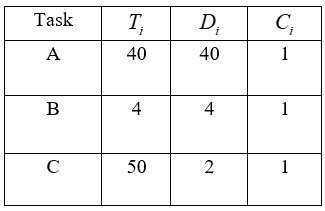
\includegraphics[scale=1]{Resources/1.png}
    	
    	\raggedright
    	الف)
    	
    	\raggedleft
    	$\sum{\frac{{{C}_{i}}}{{{T}_{i}}}}=\frac{1}{40}+\frac{1}{4}+\frac{1}{50}=29.5\%$
    	
    	\raggedright
    	ب) ابتدا ممکن است متصور شود که چون ضریب استفاده کمتر از 100 درصد می‌باشد؛ مجموعه فوق با \lr{EDF} برنامه پذیرند ولی شرط قوث برای حالتی برقرار است که 
    	$D_i = T_i$
    	برابر باشد که در اینجا برقرار نیست و باید از تست زمان پاسخ 200 ثانیه (ک.م.م) استفاده کرد که نتیجه نشان می‌دهد که مجموعه فوق با \lr{EDF} قابل برنامه ریزی هستند.
    	
    	ج)
    	
    	\raggedleft
    	$
    	DM : \sum{\frac{{{C}_{i}}}{{{D}_{i}}}}\le n({{2}^{\frac{1}{n}}}-1)\to 0.775\le 0.7798
    	$
    	
    	\lr{RM:}
    	
    	\raggedright
    	شروط کافی برای \lr{RM} نیز زمانی برقرار هستند که $D_i = T_i$ که در اینجا برقرار نیست بنابراین باید تست زمان پاسخ انجام شود.
    	
    	\raggedleft
    	
    	\begin{align}
    	\nonumber
    		&R_B = 1 < 4\\ \nonumber
    		&R_A = 2 < 40\\  \nonumber
    		&R_C = 3 > D_c =2
    	\end{align}
    	
    	\raggedright
    	با \lr{RM} برنامه پذیر نیستند.
    	
    	
    	
    	
    \end{problem}
    
    \begin{problem}{سوال دوم}
    	\centering
    	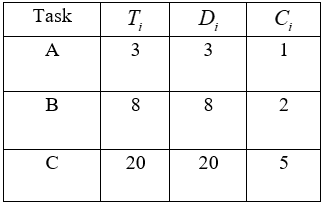
\includegraphics[scale=1]{Resources/2.png}
    	
    	\raggedleft
    	$u = 0.833 > 3(2^\frac{1}{3} - 1) = 0.7798\,\,\,\,\times$
    	
    	$\prod\limits_{i=3}^{3}{\left( \frac{{{C}_{i}}}{{{T}_{i}}}+1 \right)}=2.083>2\,\,\,\,\times $
 		
 		\raggedright
 		باید از پاسخ زمانی استفاده کنیم. اگر به صورت زمانی برنامه ریزی تحلیل شود در نهایت به پاسخ
 		$R_c = 14 < 20$
 		می‌رسیم
 		
 		نتایج بالا نشان می‌دهد که سیستم با \lr{RM} قابل پیاده سازی است.
 		
 		ب)
 		
 		\raggedleft
 		$\sum{\frac{{{C}_{i}}}{{{T}_{i}}}}=0.333+\frac{2}{{{T}_{B}}}+0.25=0.7798\to {{T}_{B}}=10.16$
 		
 		\raggedright
 		این پریود از \lr{B} که قابل برنامه ریزی بود بزرگتر است اطلاعات خاصی نمی‌دهد.
 		
 		\raggedleft
 		$\prod{\left( \frac{{{C}_{i}}}{{{T}_{i}}}+1 \right)}=2\to {{T}_{B}}=9.985$
 		
 		\raggedright
 		اگر حد بالای زمان پاسخ را با توجه به اینکه پروسه \lr{B} توسط پروسه \lr{C} قطع نمی‌شود و فقط توسط پروسه \lr{A} قطع می‌شود حساب کنیم داریم:
 		
 		\raggedleft
 		${{\overline{R}}_{c}}=\frac{5+1(1-0.333)+2(1-\frac{2}{{{T}_{B}}})}{1-(0.333+\frac{2}{{{T}_{B}}})}=20\to {{\overline{R}}_{c}}=6.346$
 		
 		\raggedright
 		البته این فرمول ها تقریبی و برای بدترین حالت هستند. آنالیز زمان پاسخ به ما جواب 
 		$T_B = 5$
 		را به عنوان کوتاهترین پریود می‌دهد.
 		
    
    \end{problem}
   

\end{document}
